%--------------------------------------------------------------------
% Эта преамбула с комментариями для написания лабораторных работ по
% физике. В еe основе информация из книги С. М. Львовского "Набор и
% верстка в пакете Latex", а также материалы по курсу "Документы и
% презентации в Latex" от ВШЭ https://www.coursera.org/learn/latex. Ну
% и мой опыт (1 год и 16 лабораторных работ + 2 Вопроса по выбору)
% Автор - Баринов Леонид
% Дата - 06.08.2019
%--------------------------------------------------------------------
%--------------------------------------------------------------------
% Для начала необходимо определиться с типом документа. Оптимальный
% (на мой взгляд) вариант - article. Также существуют типы book,
% report, proc и другие. Также в необязательном аргументе можно
% указать тип страницы и размер шрифта. Стандарт по умолчанию - А4 и
% 12 (иногда 10) шрифт. Необязательный аргумент шрифта может принимать
% только 3 параметра - 10, 11, 12 (pt).

\documentclass[a4paper, 12pt]{article}

%--------------------------------------------------------------------
% Чтобы использовать другие размеры шрифта используется пакет
% extsizes. Он позволяет указывать в \documentclass такие размеры - 8,
% 9, 10, 11, 12, 14, 17, 20 (pt). При указании других размеров могут
% возникать различные проблемы.

\usepackage{extsizes}

%--------------------------------------------------------------------
% Необходимо определиться с кодировкой документа. Идеального варианта
% для русского языка не существует - каждый чем-то немного плох. Для
% особо интересующихся - Приложение И в 5 издании книги Львовского. Я
% воспользовался вариантом, предлагаемым на курсе по Latex от ВШЭ.

\usepackage[T2A]{fontenc}
\usepackage[utf8]{inputenc}

%--------------------------------------------------------------------
% Для соблюдения типографских традиций (оказывается такие существуют)
% различных стран создан пакет babel. Самое заметное его действие -
% latex научиться переносить слова того языка, который вы укажите.
% Можно указать несколько языков через запятую. Основной язык
% документа указывается последним.

\usepackage[english,russian]{babel}

%--------------------------------------------------------------------
% Перейдем к заданию полей документа. Есть несколько способов, но
% самый простой из них - это воспользоваться пакетом geometry, который
% позволяет определить все поля документа (начиная с краев листа, что
% важно, так как некоторые другие способы позволяют это сделать только
% косвенно)

\usepackage{geometry}
\geometry{top=25mm}
\geometry{bottom=35mm}
\geometry{left=35mm}
\geometry{right=20mm}

%--------------------------------------------------------------------
% От полей логично перейти к колонтитулам. Тут нам поможет пакет
% fancyhdr. Для него существует 6 колонтитулов - верхний, левый;
% верхний, по центру; верхний, правый и такие же нижние. По умолчанию
% номер страницы находится снизу по центру, а также существует
% линейка, очерчивающие верхний колонтитул. Мне показалось интересным
% сделать колонтитулы схожие с колонтитулами в лабнике. 

\usepackage{fancyhdr}
\pagestyle{fancy}
\renewcommand{\sectionmark}[1]{\markboth{#1}{}} 
% \renewcommand{\headrulewidth}{0mm} % Если необходимо убрать линейку,
% или изменить ее длину
% \lfoot{} % Нижний левый
% \rfoot{} % Нижний правый
% \rhead{} % Верхний правый
% \chead{} % Верхний в центре
\lhead{\thepage} % Номер страницы в левом верхнем углу
\cfoot{} % Оставить нижний колонтитул без цифры

%--------------------------------------------------------------------
% Самое время научиться работать с формулами. А точнее добавить пакеты
% от Американского математического общества, которые позволять
% пользоваться большим количеством математических символов.

\usepackage{amsmath,amsfonts,amssymb,amsthm,mathtools}

%--------------------------------------------------------------------
% Также очень хочется пользоваться русскими буквами в формулах, для
% этого подключаем пакет mathtext, который добавляет окружение
% \text{}. Внутри него можно писать русские буквы в математическом
% режиме.

\usepackage{mathtext}

%--------------------------------------------------------------------
% Большим преимуществом вашего pdf документа будет возможность поиска
% в нем по словам или буквами. (Например, в Ивановнике это
% невозможно)

\usepackage{cmap}

%--------------------------------------------------------------------
% Куда же в физике без картинок и графиков? Давайте исправим
% эту недоработку

\usepackage{graphicx}
\graphicspath{images/} % Необходимо, если рисунки
% находятся в другой папке

%--------------------------------------------------------------------
% graphicx не позволяет вставлять обтекаемые рисунки, но на
% практике они очень нужны. Для этого существует пакет wrapfig

\usepackage{wrapfig}

%--------------------------------------------------------------------
% latex вставляет рисунки по определенному алгоритму. Его,
% конечно, можно менять, но это не настолько просто. Как
% правило, хочется, чтобы картинка располагалась там, где мы это
% указали в коде. Для этого существует несколько пакетов, один из
% них floatrow. Он позволяет для окружения figure указывать
% необязательный аргумент - H (именно большое h), что на latex'овском
% языке означает: вставить картинку здесь и только здесь. (даже если
% облик документа несколько пострадает)

\usepackage{floatrow}

%--------------------------------------------------------------------
% По правилам оформления рисунок всегда должен быть подписан. Для
% этого существует команда \caption{}. Но обычные настройки caption
% меня не совсем устроили. Хотелось сделать подпись меньше
% основного шрифта, а также слово Рис жирным и использовать
% разделитель точку, а не двоеточие. В этом помогает пакет,
% который называется caption (совпадение?)

\usepackage[margin=10pt,font=small,labelfont=bf,labelsep=period]{caption}

%--------------------------------------------------------------------
% Последним важным пунктом остались таблицы. Ведь куда-то нужно
% заносить результаты измерений. На данный момент во время выполнения
% лабораторных работ я заношу результаты в таблицу excel, а потом с
% помощью сайта www.tablesgenerator.com превращаю в таблицу latex и
% дооформляю.

\usepackage{array,tabularx,tabulary,booktabs}

%--------------------------------------------------------------------
% После excel есть ощущения, что везде объединить колонки или строки
% легко. В latex не совсем так. Помогают пакеты multirow, multicol. 

\usepackage{multirow}
\usepackage{multicol}

%--------------------------------------------------------------------
% Иногда могут потребоваться длинные таблицы на несколько страниц.
% Обычные таблицы latex воспринимает как одну букву. И
% становиться понятно, почему возникают проблемы при переносе
% обычной таблицы. (Ведь нельзя же перенести одну букву!). Поэтому
% вместо обычной таблицы нужна длинная таблица.

\usepackage{longtable}

%--------------------------------------------------------------------
% Часто в таблице хочется сделать перенос текста или формулы. Просто
% так это сделать не получиться из-за синтаксиса tabular. Для этого
% каждый раз необходимо создавать новое окружение tabular, что
% утомительно. Поэтому можно ввести команду \specialcell
% (назвать можно по-любому)
    
\newcommand{\specialcell}[2][c]{%
	\begin{tabular}[#1]{@{}c{}}#2\end{tabular}}

%--------------------------------------------------------------------
% Когда в таблице много колонок и строк, кажется, что они находятся
% слишком близко к друг другу. Можно переопределить
% несколько параметров, чтобы выглядело лучше. Это можно сделать либо
% в преамбуле, либо непосредственно в документе. Первое
% переопределение отвечает за интервал между строками, второе за
% интервал между колонками

% \renewcommand{\arraystretch}{1.8} 
% \renewcommand{\tabcolsep}{1cm} 

%--------------------------------------------------------------------
% В русской типографской традиции принято начинать каждый новый абзац
% с красной строки. Даже первый после заголовка (или подзаголовка).
% Чтобы каждый раз не ставить красную строку вручную существует пакет
% indentfirst

\usepackage{indentfirst}

%--------------------------------------------------------------------
% Некоторые модификаторы начертания

\usepackage{soul}
\usepackage{soulutf8}
 
\begin{document}
\thispagestyle{empty}
\begin{center}
    \textit{Федеральное государственное автономное образовательное\\ учреждение высшего образования }

    \vspace{0.5ex}

        \textbf{«Московский физико-технический институт\\ (национальный исследовательский университет)»}
\end{center}

\vspace{10ex}

\begin{center}
    \vspace{13ex}

    \so{\textbf{Лабораторная работа №_._._}}

    \vspace{1ex}

    по курсу общей физики

    на тему:

    \textbf{\textit{<<>>}}

    \vspace{30ex}

    \begin{flushright}
        \noindent
        \textit{Работу выполнил:}\\  
        \textit{Баринов Леонид \\(группа Б02-827)}
    \end{flushright}
    \vfill
    Долгопрудный \\2019
\newpage
\setcounter{page}{1}
\fancyhead[R]{\nouppercase{\leftmark}}	
\end{center}

\section{Аннотация}
В работе будут определены характеристики шарообразных неодимовых магнитов и
измерены горизонтальная и вертикальная составляющие индукции магнитного поля Земли и магнитное наклонение.
\section{Теоретические сведения}
\subsection*{Точечный магнитный диполь}
Простейший магнитный диполь может быть образован витком с током или постоянным магнитом. По
определению, магнитный момент $\vec P_m$ тонкого витка площадью $S$ с током $I$ равен:
\[
    \vec P_m = \frac{I}{c}\vec S = \frac{I}{c}S\vec n
\]
где $c$ - скорость света в вакууме, $\vec S = S\vec n$ -- вектор площади контура, образующий с
направлением тока правовинтовую систему, $\vec n$ — единичный вектор нормали к площадке $S$ (это же
направление $\vec P_m$ принимается за направление $S \to N$ от южного ($S$) к северному ($N$)
полюсу). Если размеры контура с током или магнитной стрелки малы по сравнению расстоянием до диполя,
то соответствующий магнитный диполь $\vec P_m$ называют элементарным или точечным.

Магнитное поле точечного диполя определяется по формуле, аналогичной формуле для поля элементарного
электрического диполя:
\begin{equation}
    \vec B = 3\frac{(\vec P_m, \vec r \,)\vec r}{r^5} - \frac{\vec P_m}{r^3}
\end{equation}

В магнитном поле с индукцией $\vec B$ на точечный магнитный диполь $\vec P_m$ действует механический момент сил:
\begin{equation}
    \vec M = \vec P_m \times \vec B
\end{equation}

Под действием вращающего момента $\vec M$ виток с током или постоянный магнит поворачивается так, чтобы его
магнитный момент выстроился вдоль вектора индукции магнитного поля. Это -- положение устойчивого
равновесия: при отклонении от этого положения возникает механический момент внешних сил,
возвращающий диполь к положению равновесия. В положении, когда Рт и В параллельны, но направлены
противоположно друг другу, также имеет место равновесие ($M = 0$), но такое равновесие неустойчиво:
малейшее отклонение от этого положения приведёт к появлению момента сил, стремящихся отклонить
диполь ещё дальше от начального положения.

Магнитный диполь в магнитном поле обладает энергией:
\begin{equation}
    W = -(\vec P_m,\vec B \,)
\end{equation}

Из этой формулы следует, что энергия диполя в поле минимальна и равна $W_{min} = -P_m B$ при сонаправленных
векторах $\vec P_m \upuparrows \vec B$ (угол $\theta$ между $\vec P_m$ и $B$ равен нулю), т.е., как
и следовало ожидать, в положении устойчивого равновесия.

В неоднородном поле на точечный магнитный диполь, кроме момента сил, действует ещё и сила:
\begin{equation}
    \vec F = (\vec P_m, \vec \nabla \,)\vec B 
\end{equation}
где $\vec \nabla = \left(\frac{\partial}{\partial x}, \frac{\partial}{\partial y},
\frac{\partial}{\partial z}\right)$ -- дифференциальный оператор Гамильтона.

Используя формулы для момента силы, силы и энергии, не сложно выяснить, как ведёт себя свободный магнитный диполь в неоднородном магнитном поле: он выстраивается вдоль силовых линий магнитного поля и, кроме того, под действием результирующей силы, возникающей из-за неоднородности поля, втягивается в область более сильного магнитного поля, т.е. в область, где он обладает меньшей энергией.

Зная магнитные моменты $P_1$ и $P_2$ двух небольших постоянных магнитов, можно рассчитать силу их
взаимодействия. Если магнитные моменты $P_1=P_2=P_m$ двух одинаковых небольших магнитов
направлены вдоль соединяющей их прямой, а расстояние между ними равно $r$, то магниты взаимодействуют
с силой:
\begin{equation}
    F = P_m \frac{\partial B}{\partial r} = P_m \frac{\partial(2P_m/r^3)}{\partial r} =
    -6\frac{P_m^2}{r^4}
\end{equation}

Магниты притягиваются, если их магнитные моменты сонаправлены ($P_1 \upuparrows P_2$) и отталкиваются, если моменты
направлены противоположно друг другу ($\vec P_1 \updownarrows P_2$).

Если магнитные моменты направлены перпендикулярно соединяющей их прямой, то сила их взаимодействия
окажется в два раза меньшей: $F = 3p^2/r^4$(в этом случае диполи притягиваются при $\vec P_1
\updownarrows \vec P_2$ и
отталкиваются при $\vec P_1 \upuparrows P_2$).

\subsection*{Неодимовые магнитные шары}
В настоящей работе используются неодимовые магниты шарообразной формы.
В настоящей работе имеет значение то, что:
\begin{enumerate}
\item Шары намагничены однородно;
\item Вещество, из которого изготовлены магниты, является магнитожестким материалом.
\end{enumerate}

Магнитное поле однородно намагниченного шара радиуса $R$ на расстояниях $r > R$ от центра
шара совпадает с полем точечного магнитного диполя $\vec P_m$, равного полному магнитному моменту
шара и расположенного в его центре. (Можно показать, что внутри ($r < R$) такого шара поле однородно
и равно $B_0 = 2P_m/R^3$)

Магнитожёсткость материала означает, что магнитные моменты шаров в нашей работе не изменяются под действием внешних магнитных полей, т.е. шар ведёт как жёсткий диполь. Поэтому, при расчетах можно считать, что шары взаимодействуют как жёсткие точечные магнитные диполи, расположенные в центрах шаров

Полный магнитный момент $\vec P_m$ постоянного магнита определяется намагниченностью $p_m$ вещества, из которого он изготовлен. По определению, намагниченность - это магнитный момент единицы объёма. Для однородно намагниченного шара намагниченность, очевидно, равна:
\begin{equation}
    \vec p_m = \frac{\vec P_m}{V}
\end{equation}
где $V$ -- объем шара

Намагниченность — важная характеристика вещества постоянных магнитов, определяющая, в частности,
величину остаточной магнитной индукции $B_r = 4\pi p_m$ (остаточная индукция $B_r$ — одна из величин, которая, как правило, указывается в справочниках по магнитожёстким материалам).

Не сложно показать, что индукция магнитного поля $\vec B_p$ на полюсах
однородно намагниченного шара связана с величиной намагниченности $p_m$ и остаточной магнитной
индукцией $\vec B_r$ формулой:

\begin{equation}
    \vec B_p = \frac{8\pi}{3}\vec p_m = \frac{2}{3} \vec B_r
\end{equation}

\section{Оборудование}
12 одинаковых неодимовых магнитных шариков, тонкая нить для изготовления крутильного маятника,
медная проволока диаметром ($0,5 - 0,6$) мм, электронные весы, секундомер, измеритель магнитной
индукции АТЕ-8702, штангенциркуль, брусок из немагнитного материала ($25\times 30\times60$ мм$^3$), деревянная
линейка, штатив из немагнитного материала; дополнительные неодимовые магнитные шарики ($\sim 20$ шт.) и
неодимовые магниты в форме параллелепипедов ($2$ шт.), набор гирь и разновесов.
\section{Результаты измерений и обработка результатов}
Проведем измерения массы шариков. n - количество шариков
\begin{table}[H]
\centering
\begin{tabular}{|c|c|c|}
\hline
$n$  & $m, \text{г}$      & $m_0, \text{г}$  \\ \hline
12 & 25,9 & 2,16 \\ \hline
10 & 24,2   & 2,42 \\ \hline
\end{tabular}
\captionsetup{justification=centering}
\caption{Измерение массы грузов}
\end{table}
Усредняя получим:
\[ m_0^\text{ср} = 2,29 \pm 0,13 \ \text{г}\]
Измерим диаметр одного шарика с помощью штангенциркуля и микрометра. $D$ -- диаметр $n$ шариков
\begin{table}[H]
\centering
\begin{tabular}{|c|c|c|c|}
\hline
Микрометр    & \multicolumn{3}{|c|}{Штангенциркуль} \\ \hline
$d, \text{мм}$    & $n$  & $D, \text{см}$    & $d, \text{см}$   \\ \hline
5,98 & 12 & 7,21 & 0,6 \\ \hline
6,01 & 10 & 6,00    & 0,6 \\ \hline
6,03 & 8  & 4,80  & 0,6 \\ \hline
5,99 & \multicolumn{3}{c}{} \\ \cline{1-1}
6,00    & \multicolumn{3}{c}{} \\ \cline{1-1}
\end{tabular}
\captionsetup{justification=centering}
\caption{Определение диаметра шариков с помощью штангенциркуля и микрометра}
\end{table}
Усредним:
\[d = 6,0 \pm 0,1\ \text{мм}\]

Используя дополнительные шарики, составим цепочку из 20-30 шариков и, с помощью неодимовых магнитов
в форме параллелепипедов, подсоединим цепочку к гире и разновесам, так, чтобы общая масса системы
составила $\sim 500\ \text{г}$. Добавляя или удаляя шарики, подберем минимальный вес $F$ системы цепочки с гирей, при котором она
отрывается от верхнего шарика.

Взвесим получившуюся цепочку:
\[ M = 544\ \text{г}\]

По формуле $F_0 = F/1,08$ определим силу сцепления двух шаров:
\[ F_0 = 5\ \text{H}\]

Из формулы $F_0 = 6P_m^2/d^4$ определите магнитный момент шарика $P_m$. Оценим погрешность результата.
\[ P_m = 103,9 \pm 3,5  \ \text{эрг}/\text{Гс}\]

Вычислим значение поля на полюсах по формуле $B_p = 16P_m/d^3$:
\[ B_p \approx  7700\ \pm 460\ \text{Гс} \]
\[ B_p = 0,77 \pm 0,05\ \text {Тл}\]

Значение, измереннoe магнитометром:
\[ B_p^\text{т} = 0,6 \pm 0,2\ \text{Тл}\]

\subsection*{Определение горизонтальной составляющей магнитного поля Земли}
Исследуем зависимость периода $T$ крутильных колебаний <<стрелки>> от количества магнитных
шариков $n$. $k$ -- количество полных периодов колебаний стрелки.
составляющих <<стрелку>>. 
\renewcommand{\arraystretch}{1.2} 
\begin{table}[H]
\centering
\begin{tabular}{|c|c|c|c||c|c|c|c|}
\hline
$n$  & $t, \text{с}$     & $k$  & $T, \text{с}$ & $n$  & $t, \text{с}$     & $k$  & $T, \text{с}$    \\ \hline
3 & 19,43 & 30 & 0,65 & 7  & 15,02 & 10 & 1,50 \\ \hline
3 & 9,68  & 15 & 0,65 & 7  & 7,56  & 5  & 1,51 \\ \hline
3 & 6,06  & 10 & 0,61 & 8  & 17,36 & 10 & 1,74 \\ \hline
4 & 17,56 & 20 & 0,88 & 8  & 8,39  & 5  & 1,68 \\ \hline
4 & 12,88 & 15 & 0,86 & 9  & 15,16 & 8  & 1,90 \\ \hline
4 & 8,78  & 10 & 0,88 & 9  & 15,42 & 8  & 1,93 \\ \hline
5 & 21,61 & 20 & 1,08 & 10 & 10,85 & 5  & 2,17 \\ \hline
5 & 16,15 & 15 & 1,08 & 10 & 10,46 & 5  & 2,09 \\ \hline
5 & 10,73 & 10 & 1,07 & 11 & 11,79 & 5  & 2,36 \\ \hline
6 & 12,65 & 10 & 1,27 & 11 & 11,58 & 5  & 2,32 \\ \hline
6 & 12,72 & 10 & 1,27 & 12 & 12,93 & 5  & 2,59 \\ \hline
6 & 12,48 & 10 & 1,25 & 12 & 12,68 & 5  & 2,54 \\ \hline
\end{tabular}
\captionsetup{justification=centering}
\caption{Зависимость периода $T$ крутильных колебаний от количества магнитных шариков в стрелке}
\end{table}
По результатам в таблице 3 построим график зависимости периода $T$ крутильных колебаний от
количества магнитных шариков $n$ в <<стрелке>>. (рис. 1)
\begin{figure}[H]
    \centering
    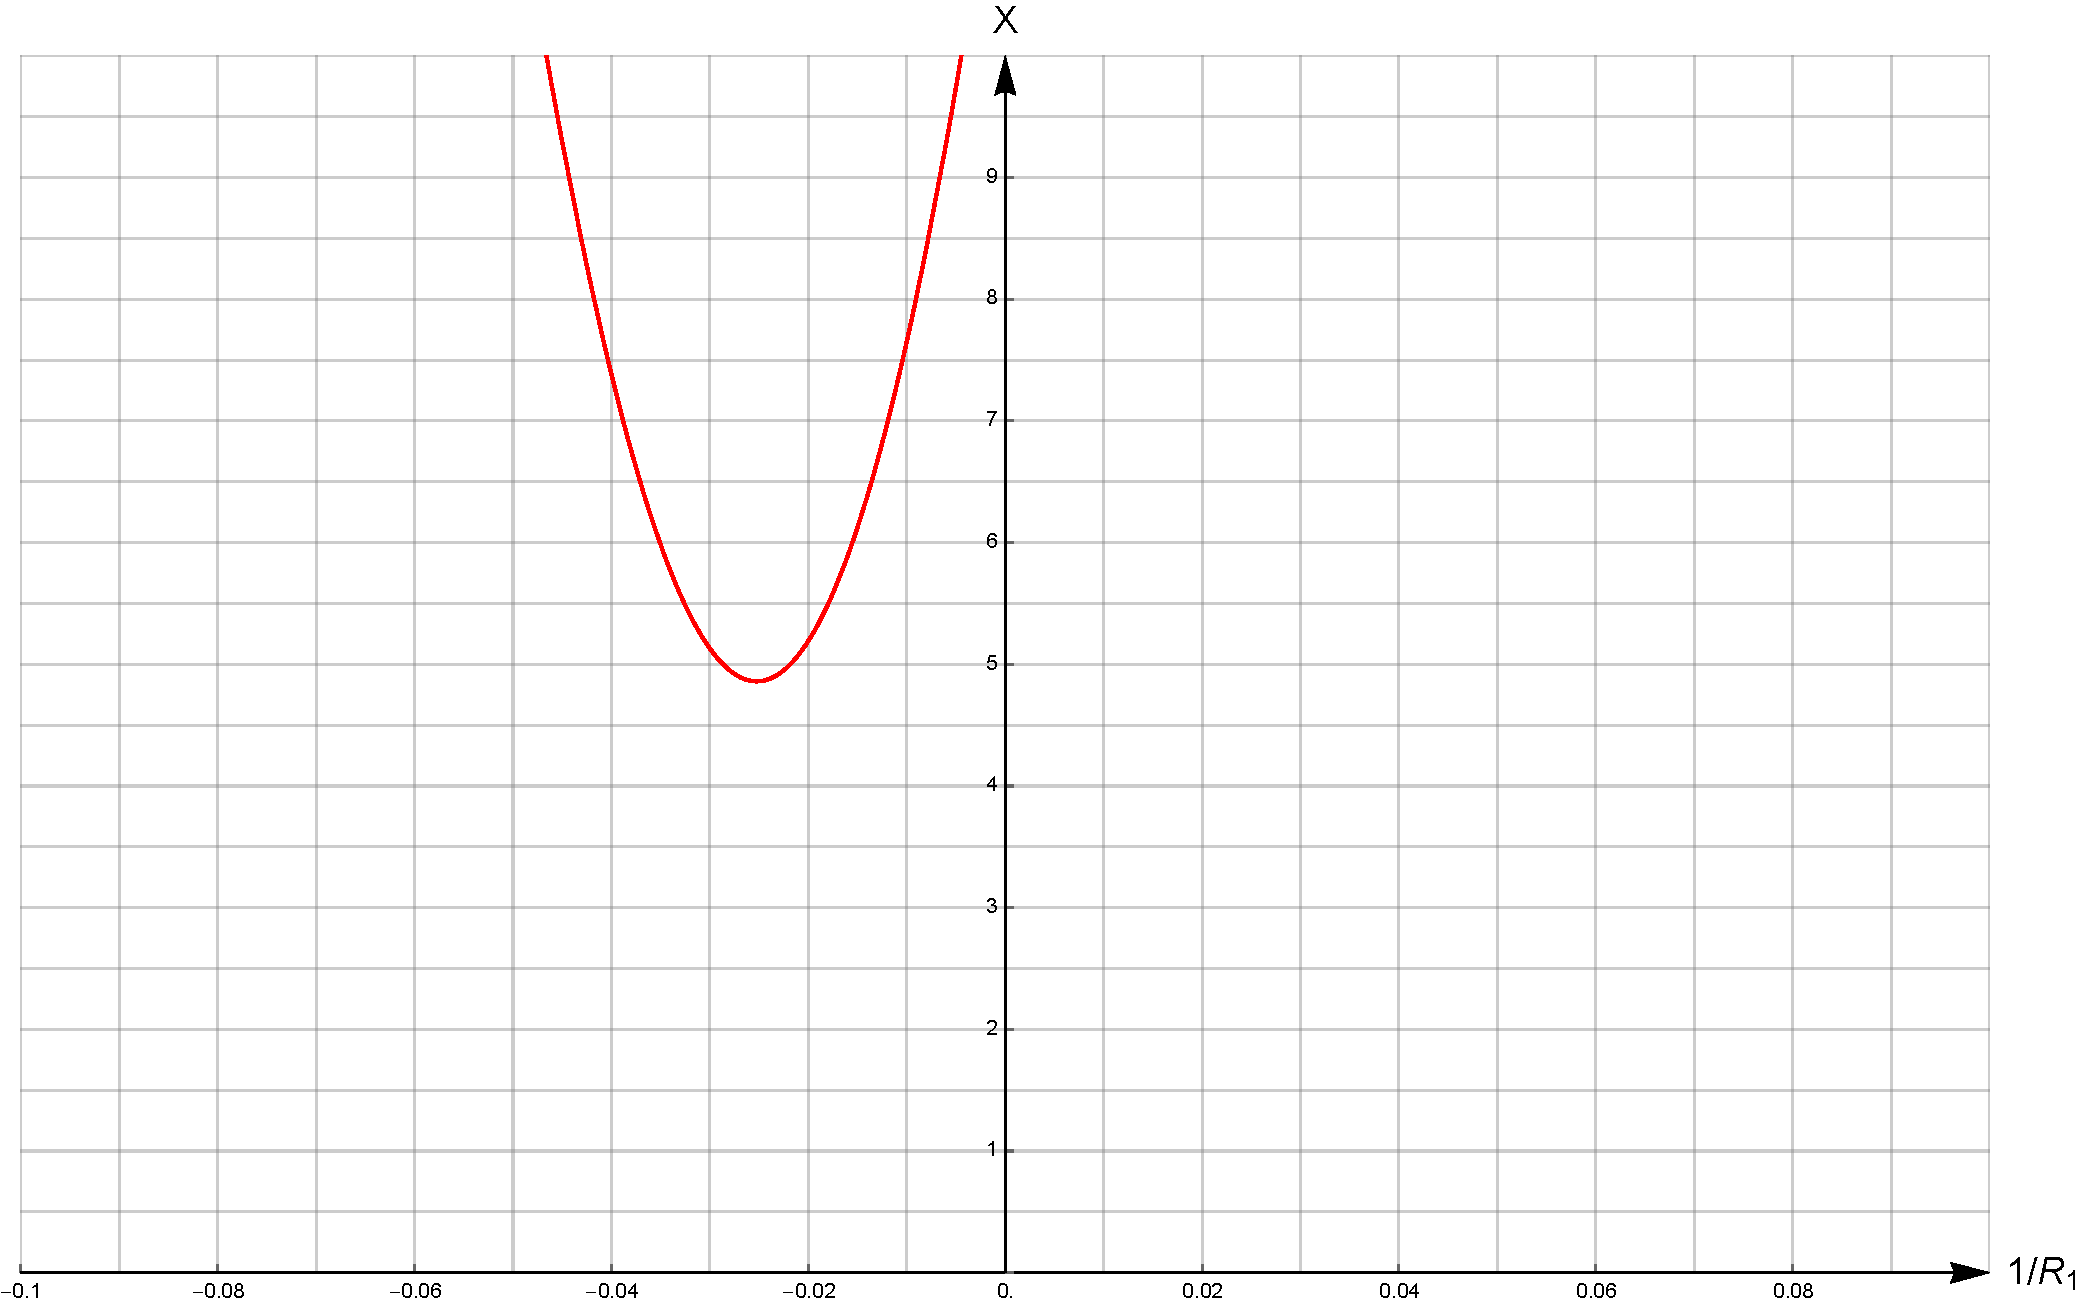
\includegraphics[width=\linewidth]{1.pdf}
    \captionsetup{justification=centering}
    \caption{график зависимости периода $T$ крутильных колебаний от
    количества магнитных шариков $n$ в <<стрелке>>}
\end{figure}

По значению углового коэффициента рассчитаем величину горизонтальной составляющей магнитного поля
Земли по формуле: $B_h = \frac{\pi^2 m d^2}{3 k^2 P_m}$ 
\[B_h = 0,58 \pm 0,04\ \text{Гс}\]

\subsection*{Определение вертикальной составляющей магнитного поля Земли}
Определим механический момент сил, действующий со стороны магнитного поля Земли на горизонтально
расположенную магнитную <<стрелку>>. Для этого, с помощью одного или нескольких кусочков проволоки,
уравновесим «стрелку» в горизонтальном положении.

С помощью весов определим массу
уравновешивающего груза $m_{\text{гр}}$. Из условия равновесия рассчитаем механический момент сил
$M$, действующих на горизонтальную «стрелку» со стороны поля Земли. $l$ -- количество шариков,
составляющих плечо силы.
\begin{table}[H]
\centering
\begin{tabular}{|c|c|c|c|}
\hline
n  & l & $m_\text{гр}, \text{г}$     & $M, \text{дин} \cdot \text{см}$   \\ \hline
\multirow{2}{*}{10} & 3 & 0,222 & 391,61 \\ \cline{2-4} 
                    & 4 & 0,131 & 308,11 \\ \hline
\multirow{2}{*}{8}  & 3 & 0,182 & 321,05 \\ \cline{2-4} 
                    & 2 & 0,281 & 330,46 \\ \hline
\multirow{2}{*}{6}  & 2 & 0,209 & 245,78 \\ \cline{2-4} 
                    & 1 & 0,348 & 204,62 \\ \hline
4                   & 1 & 0,297 & 174,64 \\ \hline
\end{tabular}
\captionsetup{justification=centering}
\caption{Зависимость момента силы $M$, действующей на горизонтальную «стрелку» со стороны поля
Земли, от количества шариков в <<стрелке>> $n$}
\end{table}
\begin{figure}[H]
    \centering
    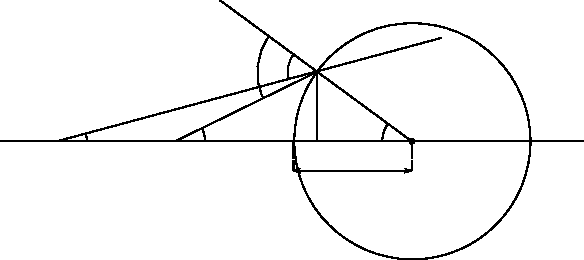
\includegraphics[width=0.79\linewidth]{2.pdf}
    \captionsetup{justification=centering}
    \caption{момента силы $M$, действующей на горизонтальную «стрелку» со стороны поля
Земли, от количества шариков в <<стрелке>> $n$}
\end{figure}
По значению углового коэффициента ($A$) вычисляем вертикальную составляющую магнитного поля Земли
по формуле $B_\nu = A/P_m$ :
\[ B_\nu  = 0,30 \pm 0,05\ \text{Гс}\]

Используя результаты измерений $B_h$ и $B_\nu$, определим магнитное наклонение $\beta$ и полную
величину индукции магнитного поля Земли на широте Долгопрудного $B$. 
     \[   \beta  \approx 27^\circ  \]
     \[   B = 0,65 \pm 0,12 \ \text{Гс}\]
Оценим также полный магнитный момент $P_\text{з}$ Земли:
\[ P_\text{З} \approx 8\cdot 10^{25}\ \text{эрг}/\text{Гс} \]

\section{Обсуждение результатов и выводы}
Была рассчитана сила сцепления двух неодимовых шаров:
\[ F \approx 5\ \text{Н}\]

В работе был определен магнитный момент неодимового шарика с диаметром $d = 6\ \text{мм}$:
\[P_m = 104 \pm 4\ \text{эрг}/\text{Гс}\quad (\varepsilon = 4\%)\]

Была расcчитана величина поля на полюсах магнитного шарика:
\[ B_p = 0,77 \pm 0,05\ \text{Тл} \quad (\varepsilon = 6\%) \]

Что в целом совпадает со значением, полученным с помощью магнитометра:
\[ B_p^\text{т} = 0,6 \pm 0,2 \text{Тл} \]

Исследована зависимость периода $T$ крутильных колебаний <<стрелки>> от количества магнитных
шариков $n$, составляющих <<стрелку>>. (Рис. 1)

По значению углового коэффициента была рассчитана величина горизонтальной составляющей
магнитного поля Земли:

\[ B_h = 0,58 \pm 0,04\ \text{Гс} \quad (\varepsilon= 7\%)\]

Результат оказался довольно сильно завышен относительно табличного значения:
\[ B_h^\text{т} = 0,15\ \text{Гс} \]

Это можно объяснить весомым влиянием других магнитов, находящихся на небольших расстояний от
установки.

Также был построен график зависимости механического момента силы $M$ от количества шариков,
составляющих магнитную <<стрелку>>. (Рис. 2)

С помощью угла наклона графика была рассчитана вертикальная составляющая магнитного поля
Земли: 
\[ B_\nu = 0,30 \pm 0,05\ \text{Гс} \quad (\varepsilon = 17\%)  \]

Что с учетом погрешности соотносится с табличным значением:
\[ B_\nu^\text{т} = 0,46 \ \text{Гс} \]

Исходя из горизонтальной и вертикальной компоненты магнитного поля Земли было определено
магнитное отклонение $\beta$ и полная величина индукции магнитного поля Земли:
\[ \beta \approx 27^\circ \]
\[ B = 0,65 \pm 0,12\ \text{Гс} \quad (\varepsilon = 18\%) \]

Видно, что значения плохо соотносятся с табличным в основном из-за рассчитанной горизонтальной
составляющей магнитного поля Земли:
\[ \beta^\text{т} = 71^\circ \]
\[ B = 0,48 \ \text{Гс}\]

Также была получена достаточно грубая оценка магнитного момента $P_\text{з}$ Земли:
\[P_\text{з} \approx 8 \cdot 10^{25}\ \text{эрг}/\text{Гс} \]

\end{document}

